\documentclass[a4paper, 12pt]{article}
\usepackage{color}
\usepackage{scalerel}
\usepackage{tikz}
\usepackage{geometry}

\geometry{
		total = {160mm, 235mm},
		left = 25mm,
		right = 25mm,
		top = 30mm,
		bottom = 30mm,
	}

\usepackage{tabularx}
\usepackage{fancyhdr}
\usepackage{graphicx}
\usepackage{amssymb}
\usepackage{amsmath}
\usepackage{multicol}
\usepackage{graphicx}
\usepackage{wrapfig}
\usepackage{enumitem}
\usepackage{lastpage}
\usepackage{transparent}
\usepackage{cancel}
\usepackage{underscore}
\usepackage{ulem}
\usepackage{listings}
\usepackage{setspace}
\onehalfspacing

\newcommand{\ans}{\textbf{Jawab} :}
\newcommand{\key}[1]{\textcolor{red}{#1}}

\begin{document}
\pagenumbering{gobble}
    \begin{tabular}{|lcl|}
     \hline
     Nama&:&Dhanar Agastya Rakalangi\\
     NRP&:&5002221075\\
     \hline
    \end{tabular}

    \begin{enumerate}
        \item 
        \begin{enumerate}
            \item Jelaskan yang dimaksud dengan inheritance, encapsulation dan 	polymorphism dalam konsep Pemrograman Berorientasi Objek\\
            
            \ans
        
            \begin{enumerate}[label=\textbullet]
                \item Inheritance : Konsep di mana sebuah class dapat mewarisi properti dan metode dari class lain.Dengan menggunakan inheritance, sebuah class dapat mengambil karakteristik dari class induknya tanpa perlu menulis ulang kode yang sama
            
                \item Encapsulation : Konsep di mana data (variabel) dan metode yang beroperasi pada data tersebut dikemas dalam sebuah class. Dengan menggunakan encapsulation, data di dalam class hanya dapat diakses dan diubah oleh metode yang ada di dalam class tersebut
    
                \item Polymorphism : Konsep di mana sebuah objek dapat memiliki berbagai bentuk atau tipe, dan dapat berperilaku berbeda tergantung konteksnya.Polymorphism memungkinkan objek dari class-class yang berbeda untuk diakses dan diproses dengan cara yang sama, sehingga memungkinkan pemrogram untuk menulis kode yang lebih fleksibel dan reusable.
            \end{enumerate}

            \item Apa yang anda ketahui tentang garbage collection dalam Java, beri penjelasan \\
            
            \ans
            
            Garbage collection merupakan proses otomatis yang dilakukan oleh Java Virtual Machine (JVM) untuk mengelola memori yang digunakan dalam program Java. Garbage collection bertugas untuk mencari dan menghapus objek-objek yang tidak lagi digunakan atau direferensikan oleh program agar memori tersebut dapat digunakan kembali.

            Proses garbage collection dilakukan dengan mengidentifikasi objek-objek yang sudah tidak terpakai dan melepaskan memori yang dialokasikan untuk objek-objek tersebut. JVM akan secara otomatis melakukan garbage collection secara terjadwal atau ketika sisa memori sudah hampir penuh.

            \item Jelaskan perbedaan method overloading dan method overriding.\\
            
            \ans
            \begin{enumerate}[label=\textbullet]
                \item Method overloading adalah kemampuan untuk mendefinisikan beberapa method dengan nama yang sama di sebuah class, namun memiliki parameter yang berbeda.
                
                \item Sementara itu, Method overriding adalah ketika subclass mendefinisikan kembali (override) method yang sudah ada di superclass dengan mengganti implementasi method tersebut.
            \end{enumerate}
            
        \end{enumerate}

        \newpage
        \item Lengkapilah potongan program berikut :\\
        \begin{figure}[h]
            \centering
            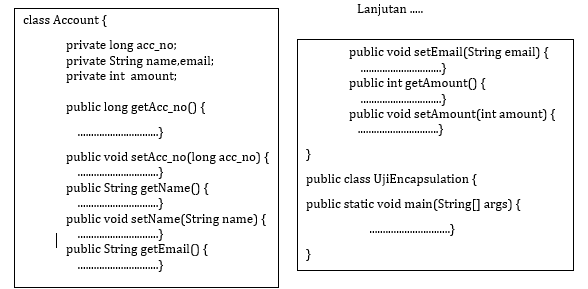
\includegraphics[width=1\linewidth]{No2.png}
        \end{figure}\\
        Agar keluaran dari program adalah sebagai berikut :\\
        \textbf{123456 Maudy Ayunda mayunda@gmail.com 50000000}\\
        
        \ans
        \begin{lstlisting}[language=Java, breaklines=true, escapeinside={$}{$}]
class Account {
    private long acc_no;
    private String name, email;
    private int amount;
        
    public long getAcc_no() {
        $\key{return acc_no;}$
    }
        
    public void setAcc_no(long acc_no) {
         $\key{this.acc_no = acc_no;}$
    }
        
    public String getName() {
         $\key{return name;}$
    }
        
    public void setName(String name) {
         $\key{this.name = name;}$
    }
        
    public String getEmail() {
        $\key{return email;}$
    }
        
    public void setEmail(String email) {
         $\key{this.email = email;}$
    }
        
    public int getAmount() {
         $\key{return amount;}$
    }
        
    public void setAmount(int amount) {
         $\key{this.amount = amount;}$
    }
}

public class UjiEncapsulation {
    public static void main(String[] args) {
        $\key{Account acc = new Account();}$
        $\key{acc.setAcc_no(123456);}$
        $\key{acc.setName("Maudy Ayunda");}$
        $\key{acc.setEmail("mayunda@gmail.com");}$
        $\key{acc.setAmount(50000000);}$
        
        $\key{System.out.println(acc.getAcc_no() + " " + acc.getName() + " " + acc.getEmail() + " " + acc.getAmount());}$
    }
}
        \end{lstlisting}
        

        \newpage
        \item Apa yang dikerjakan oleh program berikut (jelaskan tahap-demi-tahap) sehingga menghasilkan keluaran yang benar. (\textbf{HINT} : perhatikan tipe argument dari method  \textbf{cetak}.  Class Object  merupakan class tertinggi)
        \begin{figure}[h]
            \centering
            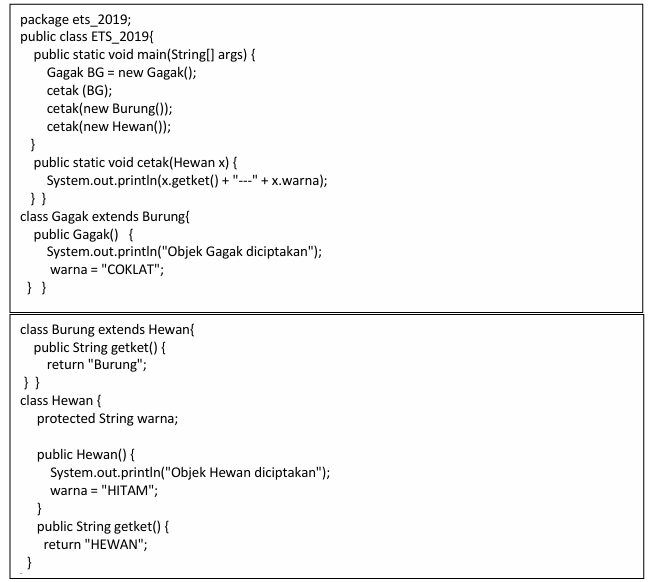
\includegraphics[width=1\linewidth]{No3.png}
        \end{figure}

        \ans
        \begin{enumerate}[label=\textbullet]
            \item Di dalam method main, pertama-tama membuat objek BG dari class Gagak.

            \item Ketika objek BG diciptakan, constructor dari class Gagak dipanggil dan mencetak "Objek Gagak diciptakan". Selain itu, nilai warna dari objek BG diinisialisasi menjadi "COKLAT".

            \item  Kemudian memanggil method cetak dengan parameter objek BG. Dalam method cetak, akan mencetak hasil dari get.ket() dari class Gagak ("Burung") dan nilai dari warna dari objek BG ("COKLAT").

            \item Selanjutnya, membuat objek baru dari class Burung tanpa nama dan langsung memanggil method cetak dengan objek tersebut sebagai parameter. Dalam method cetak, akan mencetak hasil dari get.ket() dari class Burung ("Burung") dan nilai warna dari objek tersebut (yang diinisialisasi dari constructor class Hewan dengan warna HITAM).

            \item  Terakhir, membuat objek baru dari class Hewan tanpa nama dan langsung memanggil method cetak dengan objek tersebut sebagai parameter. Dalam method cetak, akan mencetak hasil dari getket() dari class Hewan ("HEWAN") dan nilai warna dari objek tersebut (yang diinisialisasi dari constructor class Hewan dengan warna HITAM).\\

            \item[]  
            Output  :\\
            Objek Gagak diciptakan\\
            Burung --- COKLAT \\
            Objek Hewan diciptakan\\
            Burung --- HITAM \\
            Objek Hewan diciptakan\\
            HEWAN --- HITAM 
         
        \end{enumerate}

        \item Perhatikan class Diagram dalam UML berikut dengan sangat seksama. Implementasikan class diagram tersebut. Buat contoh main program dengan memanfaatkan  method-method yang ada.\\
        \begin{figure}[h]
            \centering
            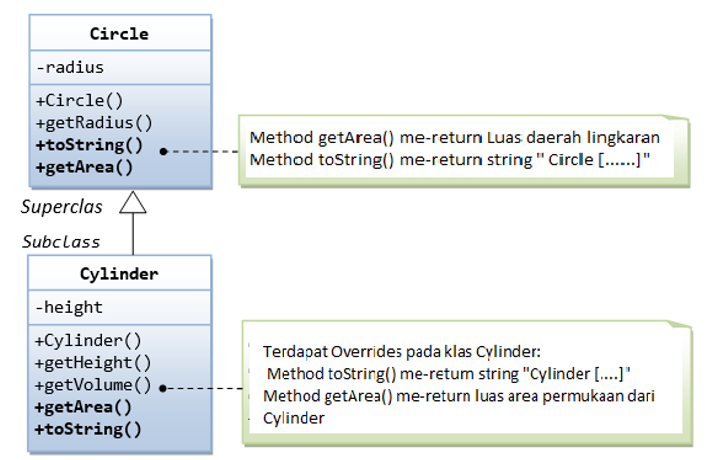
\includegraphics[width=1\linewidth]{No4.png}
        \end{figure}

         \newpage
    \ans

    \begin{lstlisting}[language=java, breaklines=true, escapeinside={$}{$}]
package Latihan_EAS_PBO;
import java.util.*;
    
public class No4 {
    public static void main(String[] args) {
        Scanner input = new Scanner(System.in);
        System.out.print("Masukkan radius: ");
        int r = input.nextInt();
        System.out.print("Masukkan height: ");
        int h = input.nextInt();
            
        Cylinder obj = new Cylinder(r,h);
        System.out.println(obj.toString());
        System.out.println("Luas Permukaan : " + obj.getArea());
        System.out.println("Volume : "+ obj.getVolume());
            
        Circle obj2 = new Circle(r);
        System.out.println(obj2.toString());
        System.out.println("Luas : " + obj2.getArea());
    }
}
    
class Circle {
    private double radius;
    
    public Circle(int x){
        radius = x;
    }
    public double getRadius(){
        return radius;
    }
    public String toString(){
        return "Circle[] dengan radius "+ radius;
    } 
    public double getArea(){
        return Math.PI*radius*radius;
    } 
}
    
class Cylinder extends Circle{
    private double height;
    public Cylinder(int x, int t){
        super(x); height = t;
    }
    public double getHeight(){
        return height;
    }
    public double getVolume (){
        return Math.PI*getRadius()*getRadius()*height;
    } 
    public String toString (){
        return "Cylinder[] dengan radius "+getRadius()+" dan tinggi "+ height;
    }
    public double getArea(){
        return 2*Math.PI*getRadius()*(getRadius()+height);
    } 
}
    \end{lstlisting}

    \item Bangunlah sebuah class bernama bilPecahan dengan spesifikasi sebagai berikut
    \begin{figure}[h]
        \centering
        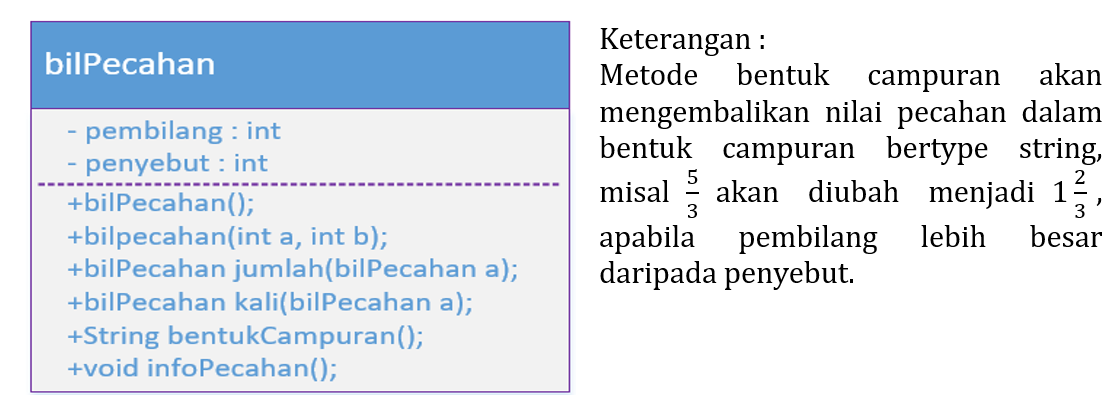
\includegraphics[width=1\linewidth]{No5.png}
    \end{figure}

    \ans

    \begin{lstlisting}[language=java, breaklines=true, escapeinside={$}{$}]
package Latihan_EAS_PBO; 
 
class bilPecahan { 
    private int pembilang; 
    private int penyebut; 
 
    // konstruktor 
    public bilPecahan(int pembilang, int penyebut) { 
        this.pembilang = pembilang; 
        this.penyebut = penyebut; 
    } 
 
    // getter 
    public int getPembilang() { 
        return pembilang; 
    } 
 
    public int getPenyebut() { 
        return penyebut; 
    } 

    
    // penjumlahan 
    public bilPecahan jumlah(bilPecahan a) { 
        int newPembilang = this.pembilang * a.getPenyebut() + this.penyebut * a.getPembilang(); 
        int newPenyebut = this.penyebut * a.getPenyebut(); 
        return new bilPecahan(newPembilang, newPenyebut); 
    } 
 
    // perkalian 
    public bilPecahan kali(bilPecahan a) { 
        int newPembilang = this.pembilang * a.getPembilang(); 
        int newPenyebut = this.penyebut * a.getPenyebut(); 
        return new bilPecahan(newPembilang, newPenyebut); 
    } 
 
    // bentuk campuran 
    public String bentukCampuran() { 
        if (pembilang >= penyebut) { 
            int integerPart = pembilang / penyebut; 
            int remainder = pembilang % penyebut; 
            return integerPart + " " + remainder + "/" + penyebut; 
        } else { 
            return pembilang + "/" + penyebut; 
        } 
    } 
 
    // setter 
    public void setPembilang(int pembilang) { 
        this.pembilang = pembilang; 
    } 
 
    public void setPenyebut(int penyebut) { 
        this.penyebut = penyebut; 
    } 
 
    // info pecahan 
    public void infoPecahan() { 
        System.out.println("Pembilang: " + pembilang); 
        System.out.println("Penyebut: " + penyebut); 
    } 
} 
$\newpage$
public class No5 { 
    public static void main(String args[]) { 
        bilPecahan p1 = new bilPecahan(3, 2); 
        bilPecahan p2 = new bilPecahan(1, 4); 
        bilPecahan hasilJumlah = p1.jumlah(p2); 
        System.out.println("Hasil Penjumlahan: " + hasilJumlah.bentukCampuran()); 
        bilPecahan hasilKali = p1.kali(p2); 
        System.out.println("Hasil Perkalian: " + hasilKali.bentukCampuran()); 
    } 
}        
    \end{lstlisting}
    
    \end{enumerate}

   
\end{document}
